\documentclass[UTF8]{ctexart}
\usepackage{graphicx}
\usepackage{amsmath}
\pagestyle{plain}   
% \usepackage{booktabs}
% \usepackage{subfigure}
\usepackage{setspace}
\date{}
\title{Bloom Filter 实验报告} 
\author{杨景凯}
\date{2021/3/7} 
\begin{document} 
% \maketitle 
\begin{center}
    \quad \\
    \quad \\
    \quad \\
    \vskip 3.5cm
    \heiti \zihao{1} Bloom Filter 实验报告\\
\end{center}
\vskip 3.5cm
\begin{quotation}
    \songti \fontsize{30}{30}
    \doublespacing
    \par\setlength\parindent{12em}
    \quad 
\begin{center}
    %学\hspace{0.61cm} 院:\underline{电子信息与电气工程学院}

    学生姓名:\underline{\qquad    \quad \quad 杨景凯    \quad  \quad\qquad }

    学\hspace{0.61cm} 号:\underline{\quad \quad\quad520021910550\quad\quad}

\end{center}
    
    \centering
    2022年3月7日
\end{quotation}
\clearpage
\tableofcontents
\clearpage
\section{实验思路}
\subsection{对数据的分析}
对于本次实验,输入数据具有的特点是:数量少、随机性差。
\subsection{哈希函数的选取}
根据输入数据的随机性差的特点,我先后选取了以下三种哈希函数,并最终选取了最后一种哈希函数。
\subsubsection{使用C++库中的std::hash}
std::hash具有较大的避免哈希冲突的可能性,但是其对于int类型的数据仅为映射到其本身,而对于此次实验的数据来说,不具有较大的随机性。只能将数据映射到本身使得哈希表没有意义。
\subsubsection{使用自己写的哈希函数}
在放弃使用C++库中的std::hash后,我尝试自己写哈希函数。根据质数不容易冲突的性质,我在100的附近取得一些质数,将其相乘后对总空间取余,如下图所示。
\begin{center}
    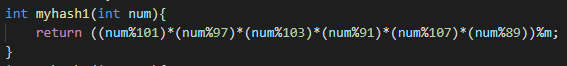
\includegraphics[scale=0.7]{hash1.png}
\end{center}
在使用此哈希函数测试时,发现最终结果依旧不满意,由于原来的数据取模后大多不发生变化,故随机性依旧不好。导致结果不佳。
\subsubsection{采用随机性更强的哈希函数}
如果是为了更好的随机性,那么为什么不去使用随机数呢?因此我采用了下面图片所示的哈希函数,进行了最终的实验。
\begin{center}
    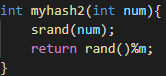
\includegraphics[scale=1.2]{hash2.png}
\end{center}
\section{实验过程}
\subsection{实验说明}
实验中,待插入的数据为0到99,检验的数据为100到199,对于不同k,不同哈希函数为产生微小变化。如果$H_2(x)=H_1(x+1)$,那么因为数据的连续性(较差的随机性),那么只有最后的多次哈希起作用。因此我采用$H_j(x)=H_1(x \cdot j)$,其中$j$是哈希函数的序数。
\section{实验结果}
\subsection{实验表格}
实验结果如下表所示:
\begin{table}[hp]
    \centering
    \textbf{实验结果表格}\\
    \begin{tabular}{|c|c|c|c|c|}
        \hline
        m/n& 2&	3&	4&5\\
        \hline
        k&	1.386294&	2.079442&	2.772589&3.465736\\
        \hline
        k=1&	0.15&	0.53&	0.4&0.31\\
        \hline
        k=2&	0.39&	0.24&	0.24&0.18\\
        \hline
        k=3&	0.43&	0.03&	0.18&0.18\\
        \hline
        k=4&	0.53&	0.09&	0.26&0.08\\
        \hline
        k=5&	0.59&	0.11&	0.35&0.03\\
        \hline
    \end{tabular}
\end{table}
\newpage
\subsection{实验结果分析}
观察表格,我们可以发现,在m/n=2,3,4时结果与理论相接近,符合。但是在m/n=5时存在问题。理论上,最小值应该在3与4之间,但是实验结果显示在5处最小。我向后测试了m/n=6的结果,发现是增加的。因此是稍微有所偏差。考虑到输入数据的连续性(较差随机性)以及多哈希函数的重叠,结果存在偏差。
\subsection{实验结论}
根据上述实验,我们可以验证BloomFilter在$k=\ln 2 \cdot (m/n)$时误报率最低,理论成立。


\end{document}
